\documentclass[authorontitle=true]{bfhbeamer}
\usepackage{amsmath}
\usepackage{pgfpages}

\setbeamertemplate{page number in head/foot}[framenumber]
\title{Decibel Threshold Event Displayer}
\subtitle{BTI3031 Project 1 | Final Presentation}
\author{Dominic Gernert, Lukas von Allmen, Darius Degel}

% macro which adds fancy ToC to all sections
\AtBeginSection[]
{
  \begin{frame}
    \frametitle{Table of Contents}
    \begin{columns}
      \column{0.6\textwidth}
        \tableofcontents[
            sectionstyle=show/shaded,
            subsectionstyle=show/show/hide
        ]
      \column{0.4\textwidth}
          \includegraphics[width=0.6\textwidth]{../assets/ear.png}
    \end{columns}
  \end{frame}
}

\begin{document}
%\pgfpagesuselayout{2 on 1}[a4paper, border shrink=5mm]
\maketitle
\section{Problem Description}\label{sec:problem-description}
% ---------------------------------------------------------------------------
% Initial Situation
\begin{frame}
    \frametitle{Initial Situation}
    \centering
    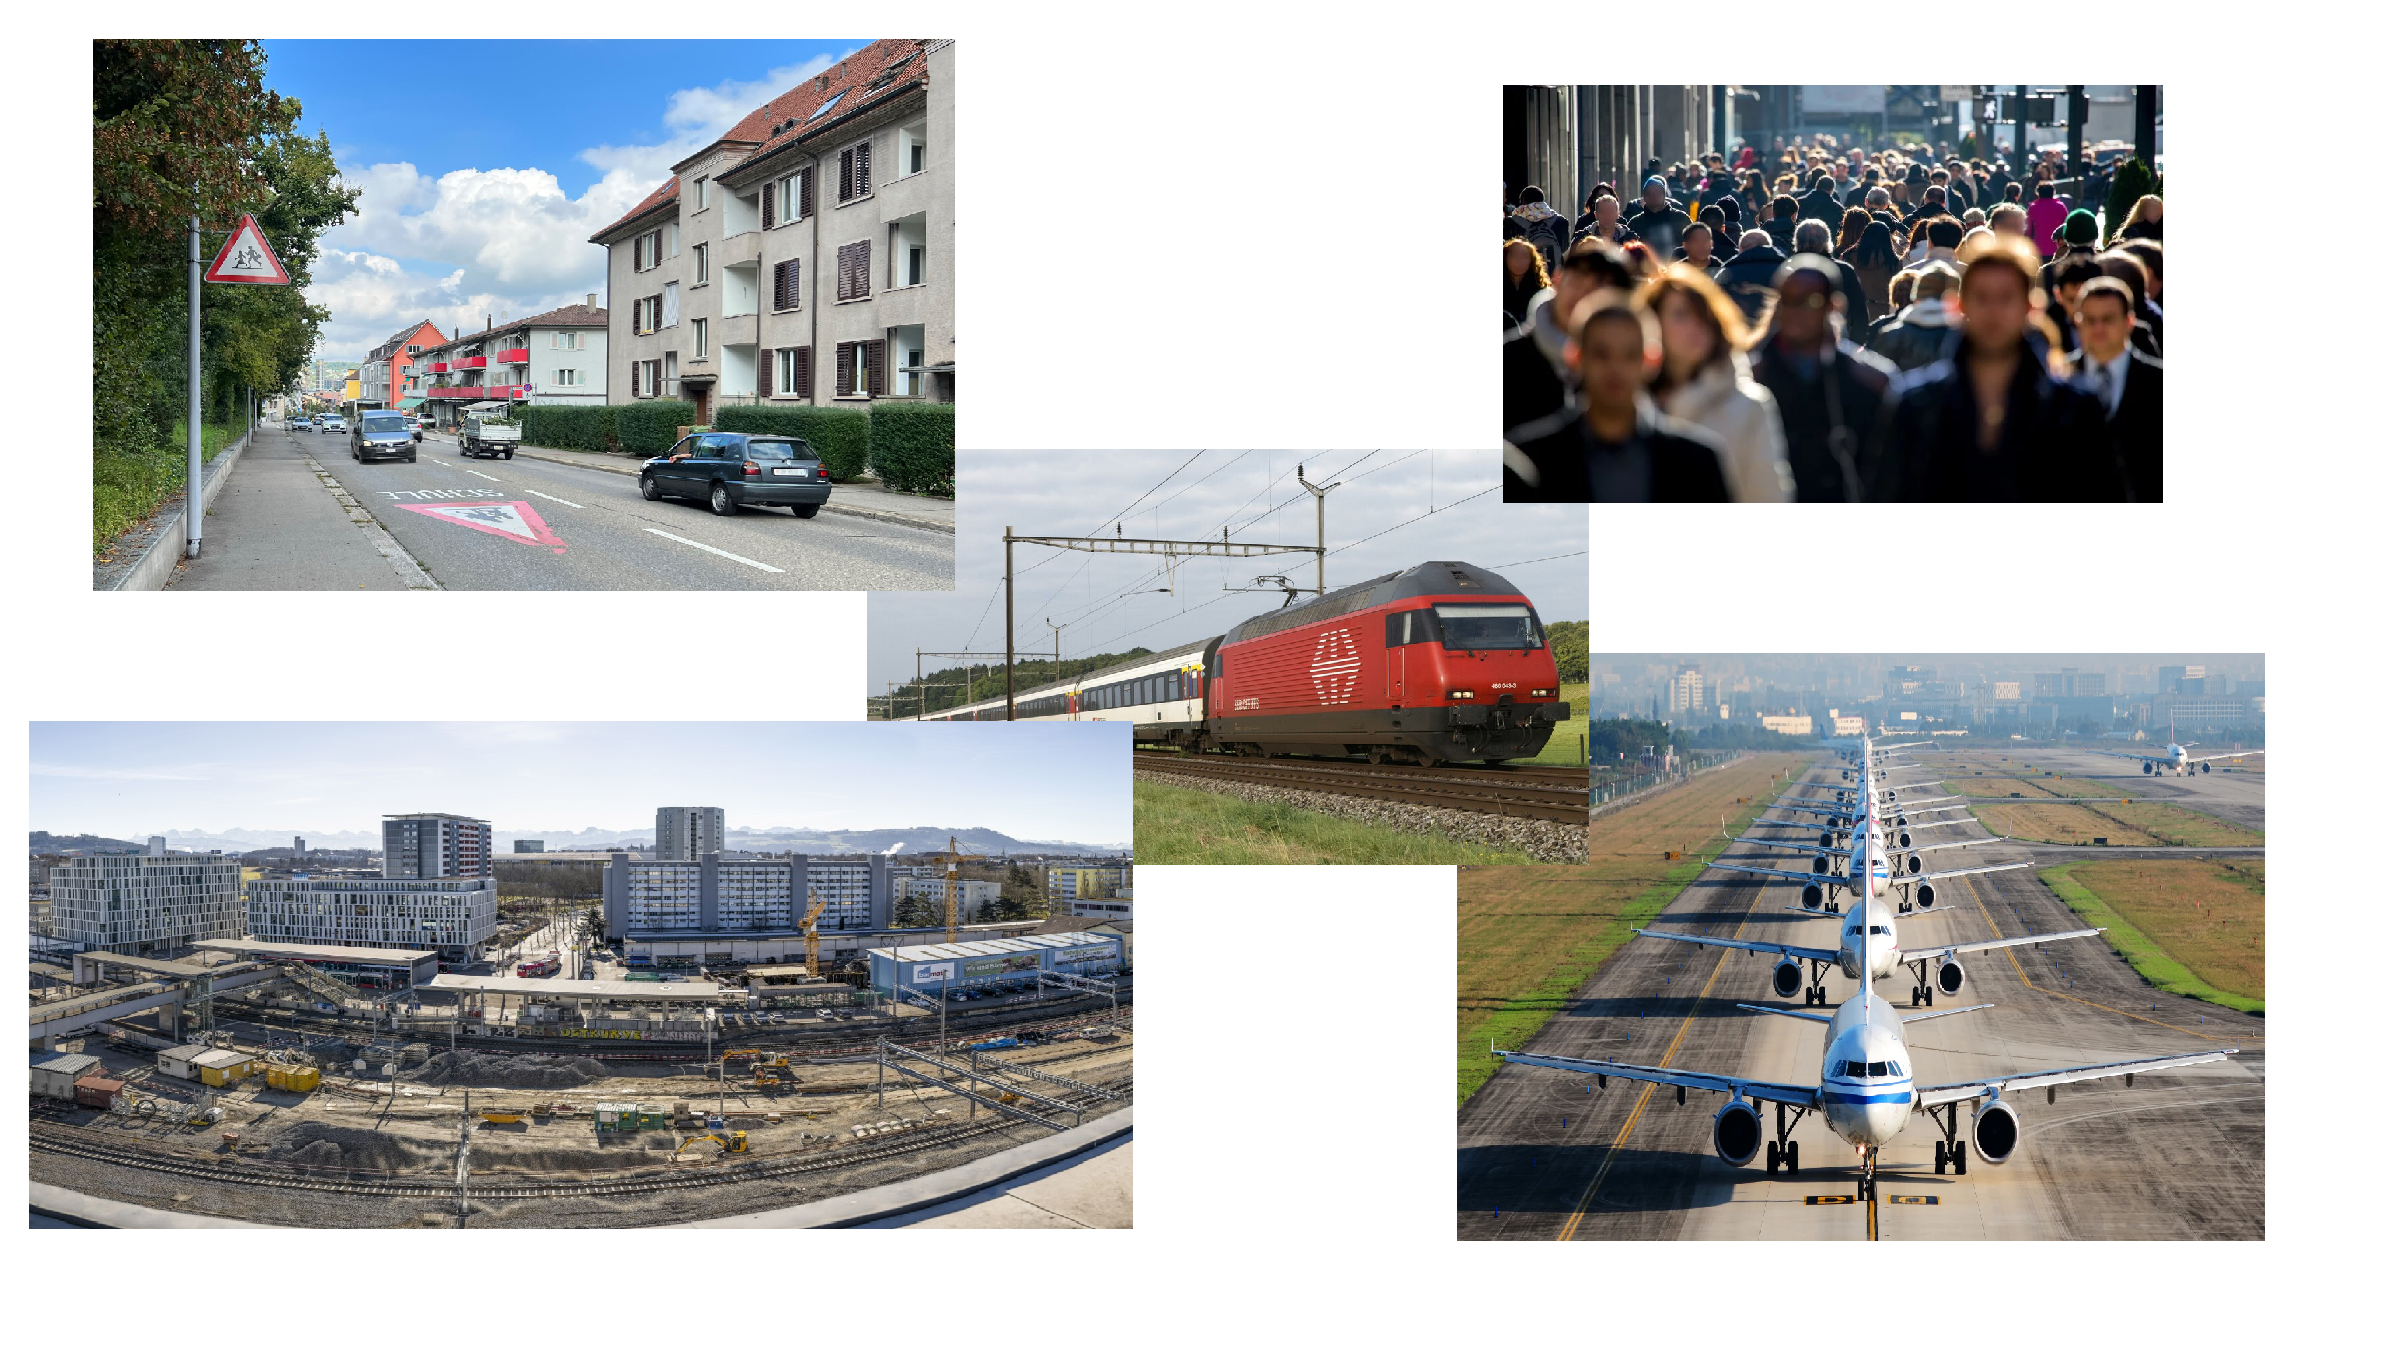
\includegraphics[width=0.8\linewidth]{../assets/collage_sound_pollution.png}
\end{frame}
% ---------------------------------------------------------------------------

% ---------------------------------------------------------------------------
% Project Goals
\begin{frame}
    \frametitle{Project Goals}
    \begin{itemize}[<+->]
        \large
        \item Analyze Audio File
        \item Summarize findings in a PDF
        \item Easy to use
    \end{itemize}
\end{frame}
% ---------------------------------------------------------------------------

% Requirements
\begin{frame}
    \frametitle{Requirements}
    \begin{columns}
        \column{0.5\textwidth}
        \begin{itemize}[<+->]
            \large
            \item Take Wave File and Threshold as Input
            \begin{itemize}
                \large
                \item and additional Reference values
            \end{itemize}
            \item Analyze and Summarize 
            \begin{itemize}
                \large
                \item Metadata
                \item Plot
                \item Render with LaTeX
            \end{itemize}
            \item User should not need any Technical know-How
            \item Multiple Languages
        \end{itemize}
        \column{0.5\textwidth}
        \includegraphics[width=0.8\linewidth]{../assets/min_and_max_measuring.png}
    \end{columns}
\end{frame}
% ---------------------------------------------------------------------------
\section{Implementation}\label{sec:implementation}
% ---------------------------------------------------------------------------
% Privacy/License
\begin{frame}
    \subsection{Privacy / License}\label{subsec:privacy-and-license}
    \frametitle{Privacy / License}
\end{frame}
% ---------------------------------------------------------------------------

% ---------------------------------------------------------------------------
% Architecture
\begin{frame}
    \subsection{Architecture}\label{subsec:architecture}
    \frametitle{Architecture}
\end{frame}
% ---------------------------------------------------------------------------

% ---------------------------------------------------------------------------
% Processes
\begin{frame}
    \subsection{Processes}\label{subsec:processes}
    \frametitle{Processes}
\end{frame}
% ---------------------------------------------------------------------------

% ---------------------------------------------------------------------------
% Testing
\begin{frame}
    \subsection{Testing}\label{subsec:testing}
    \frametitle{Testing}
\end{frame}
% ---------------------------------------------------------------------------

% ---------------------------------------------------------------------------
% Deployment / Distribution
\begin{frame}
    \subsection{Deployment / Distribution}\label{subsec:deployment-and-distribution}
    \frametitle{Deployment / Distribution}
\end{frame}
% ---------------------------------------------------------------------------

\section{Scrum}\label{sec:scrum}
\begin{frame}
    \frametitle{Scrum}
    \begin{itemize}
        \large
        \item 2 week iterations
        \item Daily every week
        \item Review / planning every other week
        \item Product goals / sprint goals
        \item GitLab, MS Teams, LaTeX, excalidraw, draw.io
    \end{itemize}
\end{frame}
\section{Demo}\label{sec:demo}
\begin{frame}
    \frametitle{Demo}
\end{frame}
\section{Conclusion \& Future Work}\label{sec:conclusion}
\section{Conclusion}
This was the first time that anyone of us has worked that much with audio files. We learned a lot about how audio overall works and how to process it. We learned especially a lot about how the wav file format or rather the riff format family works, because we implemented our own parser for that. As in every project there were some challenges we encountered in the course of the semester, but we never had the feeling that we were not in control of the situation. We are pleased with how we managed the project and the outcome of the project. To implement it as webbased application was a good decision, as the user does not need to install anything and it is accessible from everywhere. This way we can reach the miximal number of potential users. We think that our application provide some real value for people affected by noice disturbance, because they have the possibility to create a full noice report with an easy to use website.

\subsection{Review}
We initialy struggled with the task of filtering the audio with a given threshold. This was due to the fact that the audio samples in wav files represent relative loudness and not absolute. And to filter the audio we need absolute values. After researching we found out that we can map the values from the samples to absolute ones when we have some reference values. 
We also had issues with the implementation of the parsing of individual samples because of the way that javascript handles numberic values. In the end we were able to fix this by using the appropriate functions to read bytes. Besides does minor difficulites, we did not encounter any issues which could endanger the achievement of our targets. 
The project management with Scrum gave a noticable overhead for the whole project and we spent a good amount of time every week to hold the scrum meetings. We think that this was a bit to much for a project of this size. But never the less it helped us to manage and prioritize our tasks and to focus on independent features to implement. 
From a documentation perspective it was the largest project that we have used latex for. We learned alot about how to setup the a document and discovered some new packages and tricks along the way. It was also the first time that we used latex instead of powerpoint for our presentation.

\subsection{Bottom Line}
It is hard to quantify how much time is saved by using our application. There already exist other application which do a similiar thing as ours. The value of our application lies in the creation of a full noice report, because there are a ton of websites for just analyzing a wav file. So we assume that it would take the average person around 15 minutes to combine all information necessary in a word document and format it to look like some kind of report. With our application it takes less then 2 minutes to fill in the form and create the pdf. So we estimate that there is a time saving of around 13 minutes when using our application. Of course we have to consider that someone can reuse a previously in word created noice report, so he only has to gather the information and fill it in. We assume that this takes the user around 5 minutes, so in that case the saving would be only around 3 minutes per noice report.

\subsection{Future Work}
The most obvious next step for the project would be to support multiple languages, so that we can reach more people. We would also like to implement a way for the user to declare custom thresholds to select from, basically some kind of "favorites" list for thresholds. Additionally it would be convenient to add custom form fields which would be added to the noice report, in case some other information would be missing. From a technical perspective we only support the wav file format, and from that only a subset of the most common sample encoding formats. It would be nice to also support others like mp3 or aac. Also the latex dependency management could be improvement. Because we preload the latex dependencies, we need a list of all of them. The creation of that list is currently a manual process.
\end{document}